\chapter{Umsetzung und Implementierung}

\section{Software}

requirements.txt kann im Anhang gefunden werden mit der vollständigen Liste.

\begin{itemize}
    \item Virtual Python environment.
    \item Implementiert in Tensorflow. (angefangen in version 1.8, später nach 1.11 upgedatet)
    \item Datenhandling: mit Pandas. Da Data Science ein wichtiger Part der Arbeit war, sehr wichtig erwähnen
    \item Matplotlib für Visualisierung (die meisten selbstgemachten grafiken hier in der Arbeit)
    \item OpenCV für Bilderdinge in der Pipeline (wie oben erwähnt)
    \item MATLAB, für Tracksort und die Ursprünglichen implementation der Vergleichsdinge für evaluationen 
\end{itemize}

\todo[inline]{Aufpassen dass das nicht zu viel wird}

\section{Code Struktur}

Vorgehen beschrieben in \ref{CodeStruktur}.
\todo[inline]{überlegen wie viel ich überhaupt dazu schreiben soll - }

\begin{figure}
    \centering
    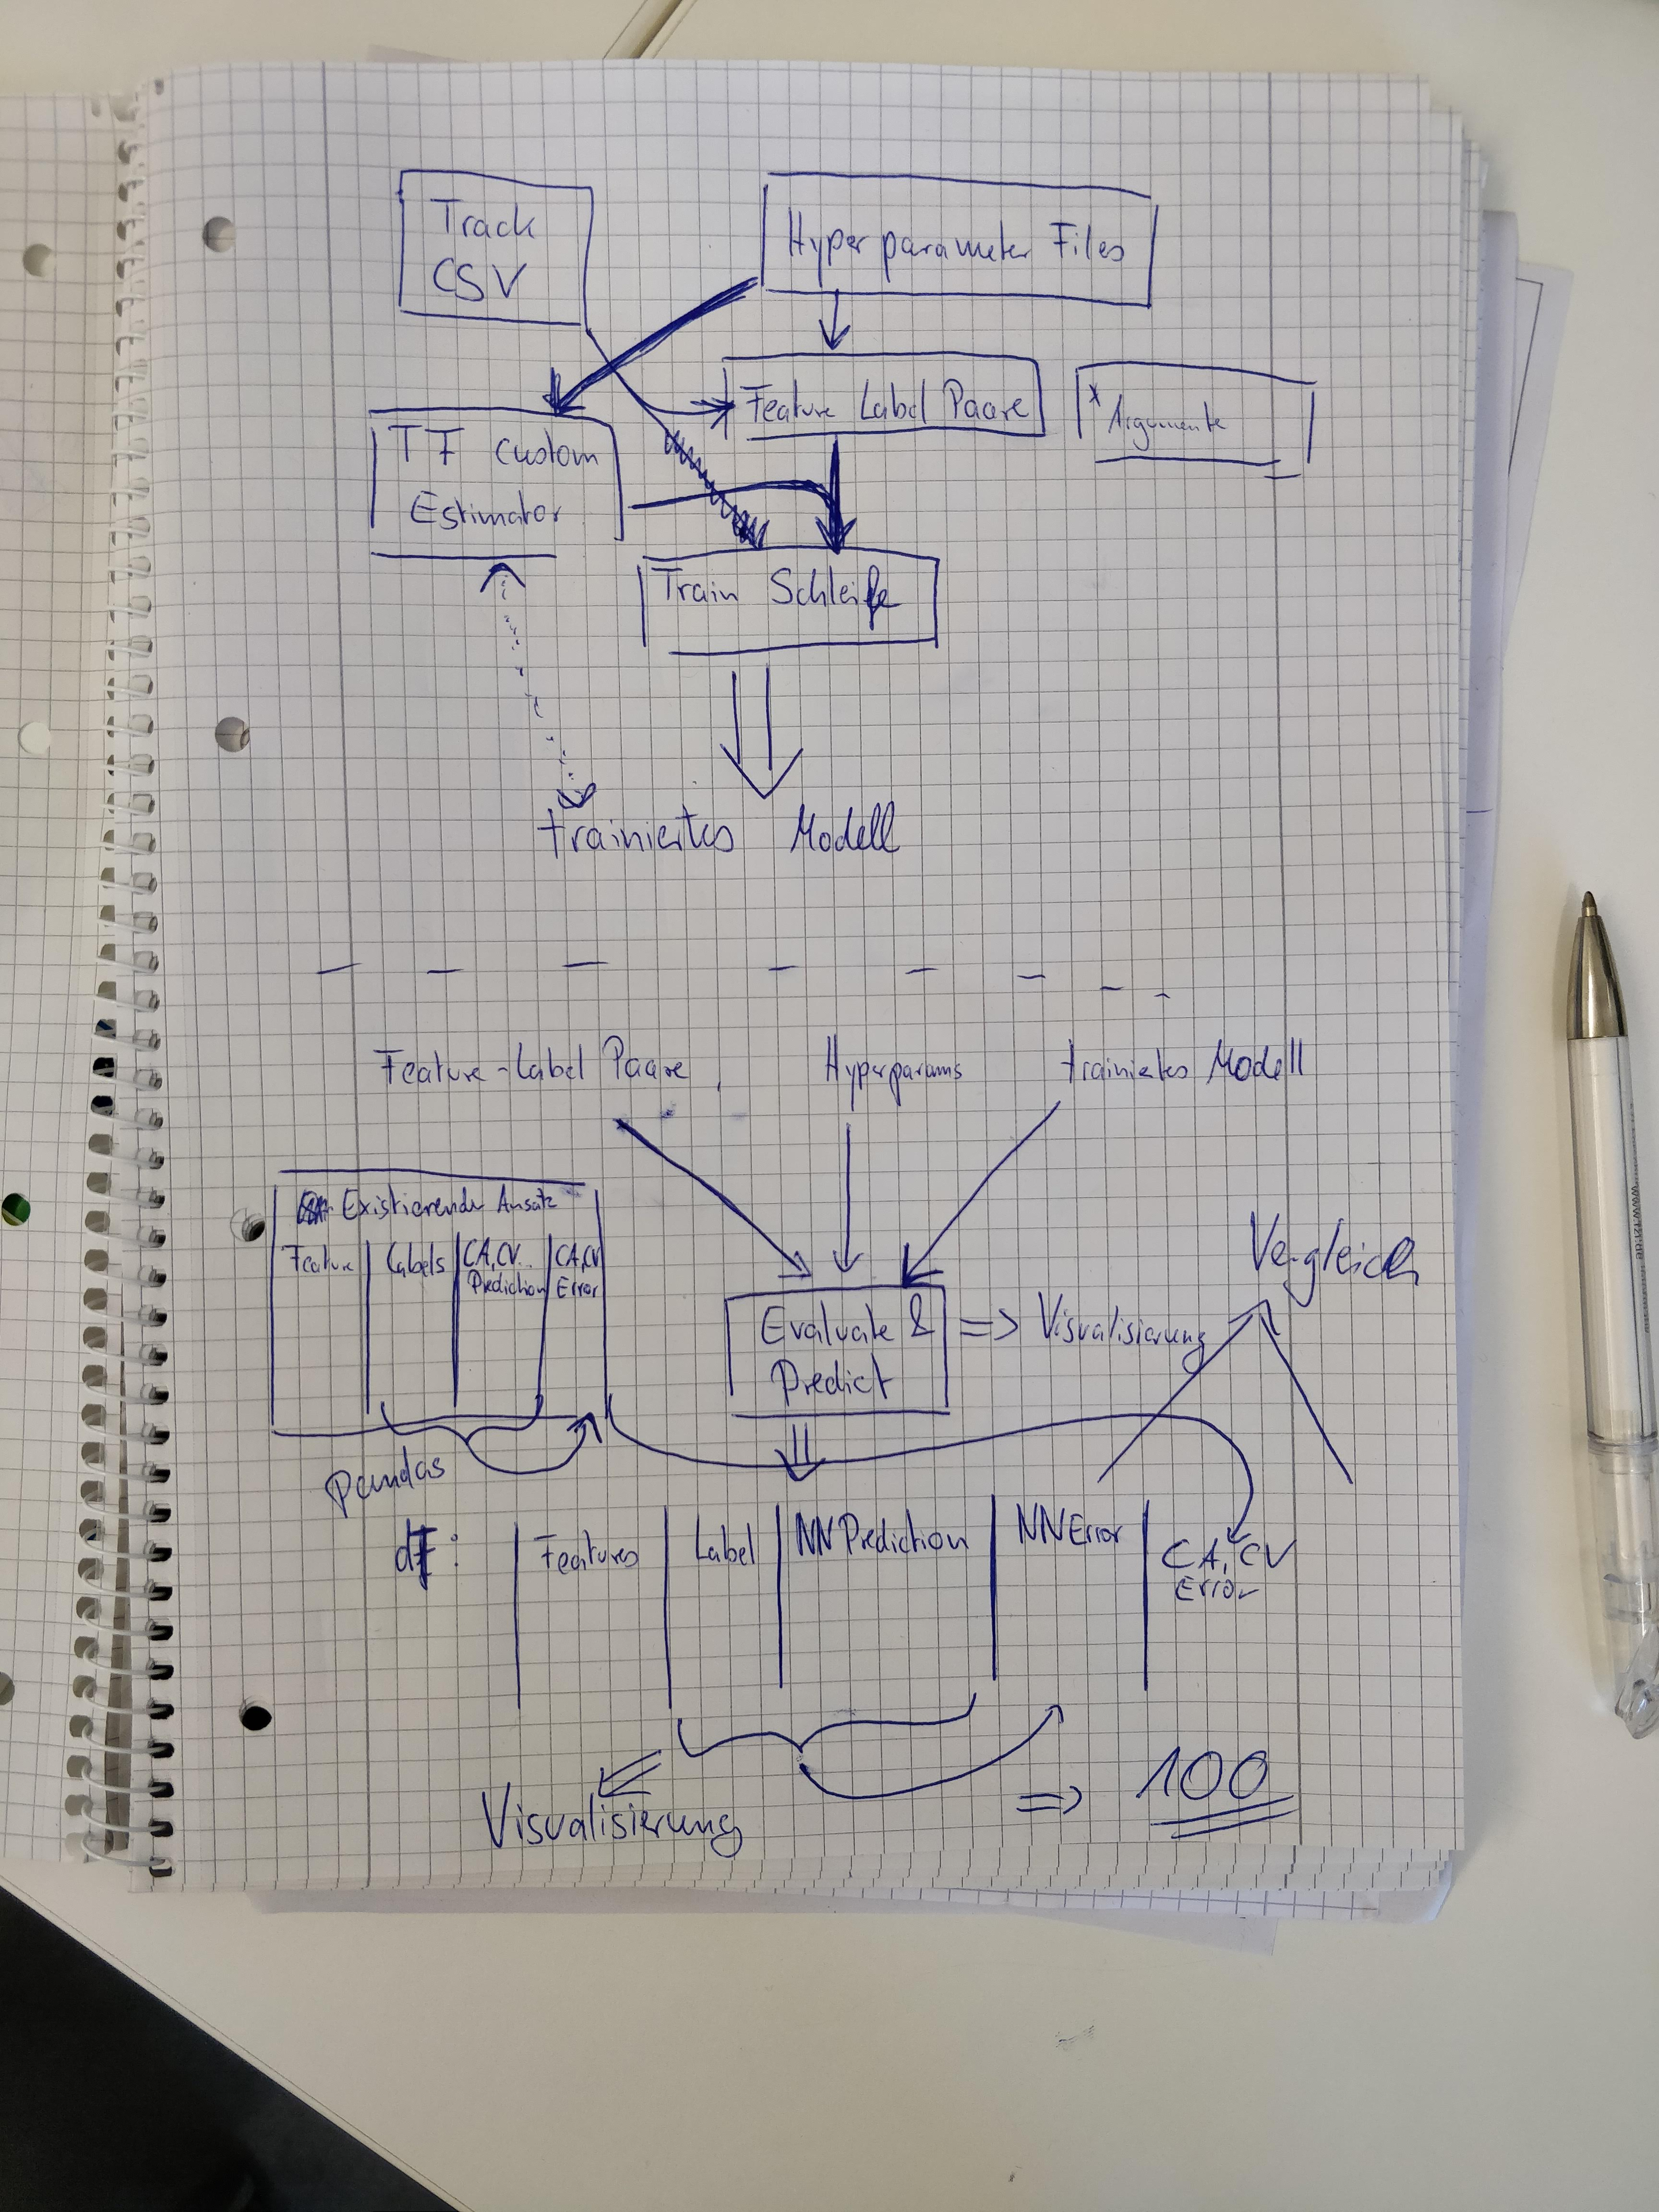
\includegraphics[width=\textwidth]{CodeStrukturSkizze}
    \caption{Skizze Codestruktur}
    \label{CodeStruktur}
\end{figure}
  

\section{Hyperparameter}

Hyperparameter sind die Variablen, die die Struktur des Netzes bestimmen (Eg: Anzahl Layers, FeatureSize) 
sowie die Variablen, die festlegen wie das Netz trainiert (z.B. Lernrate, Anzahl Epochen)
 determine how the network is trained(Eg: Learning Rate).

Hyperparameters are set before training(before optimizing the weights and bias).

\noindent\begin{minipage}{\textwidth}
\begin{lstlisting}[language=json,firstnumber=1, caption={Beispiel eines Hyperparameter Files in JSON}, captionpos=b, label=lst-hyperparam]
    {
        "arch": {
            "dropout_rate": 0.0,
            "hidden_layers": [16, 16, 16],
            "feature_size": 5,
            "activation": "leaky_relu"
        },
        "problem": {
            "data_path": "/home/hornberger/MasterarbeitTobias/data/simulated/SpheresDownsampled",
            "modelBasePath": "/home/hornberger/MasterarbeitTobias/models/simulated/",
            "imagePath": "/home/hornberger/MasterarbeitTobias/images/",
            "separator": 0,
            "separatorPosition": 1550,
            "thresholdPoint": 1200,
            "predictionCutOff": 1300

        },
        "train": {
            "batch_size": 1000,
            "epochs": 500,
            "steps_per_epoch": 200,
            "learning_rate": 0.01,
            "optimizer": "Adam"
        },
        "data": {
            "numberFakeLines": 500,
            "testSize": 0.1,
            "augmentMidpoint": 1123,
            "augmentRange": 1000,
            "direction": "x",
            "unitLoc": "px",
            "unitTime": "1/100 Frames",    
            "limits": [0.388, 0.788, 0.0, 0.18]
        }
    }

    
\end{lstlisting}
\end{minipage}
    
\begin{itemize}
\item Architektur:
    \begin{itemize}
        \item Dropout: Wahrscheinlichkeit für das zufälliges ausschalten von einzelnen Neuronen
        \item Hidden Layer: ein Array an Zahlen repräsentiert die Architektur der Hidden Layers. Jede Zahl ist ein FC Layer mit so vielen neuronen
        \item FeatureSize: Wie viele Positionen bekommt das Netz als Input ( => Größe des Inputlayers = 2x FeatureSize)
        \item Activation: Aktivierungsfunktionen für die neuronen der Hidden Layers
        % - optionen: "relu", "leaky_relu", "linear"
    \end{itemize}
\item Problem:
    \begin{itemize}
        \item DataPath: wo liegen die CSV Dateien zum die Daten rausladen
        \item ModelPath: wo soll das Netz hingespeichert werden/Hergeladen - mit Checkpoints usw.
        \item ImagePath: wo sollen Bilder hingespeichert werden, z.B. von Plot
        \item separator: 0 oder 1, jenachdem ob es den nächsten Schritt (0) oder zum Düsenbalken (1) prädizieren soll
    \end{itemize}

    Falls Separator 1:
    \begin{itemize}
        \item separationPosition: Koordinate des Düsenbalken und Ziel der Prädiktion
        \item ThresholdCutoff \todo{verify}
        \item predictionCutOff: Koordinate hinter der keine FeatureTupel mehr genommen werden
    \end{itemize}
\item Train:

\end{itemize}


\subsection{Hyperparameter Tuning}

Als Hyperparameter Optimierung oder auch Hyperparameter Tuning bezeicht man den Vorgang das am besten geeignete Set an 
Hyperparametern für einen Lernalgorithmus zu wählen.


Vorgehen bei dieser Arbeit: Jeweils für NextStep und für Separator getrennte Konfigurationen finden.

Suchen auf Simulierten Daten und dann auf allen Daten verwenden.



Aktueller Stand:
NextStep: kein Overfitting gefunden => L1 und L2 Regularisierung haben keinen positiven Effekt
Adam Optimizer ist am besten
leaky\_relu reigns supreme
Learning Rate Decay ist eine gute Idee. (Höherer Wert => langsamerer Zerfall)
FeatureSize 5 ist gut, weniger wird schlechter und Mehr ist auch schlechter geworden (potenziell weil weniger Beispiele?)

Separator: 

\subsection{Architektur des neuronalen Netzes}

Input layer: \(2 * FeatureSize\) Neuronen

\(N\) hiddenlayer (as determined by Hyperparameter tuning) mit jeweils \(m\) Neuronen.
Fully connected!

Output layer:
Linear activation weil regression.
2 Neuronen, eins für die eine Label Dimension und eins für die andere.

\begin{figure}
    \centering
    % \missingfigure{Grafik architektur}
	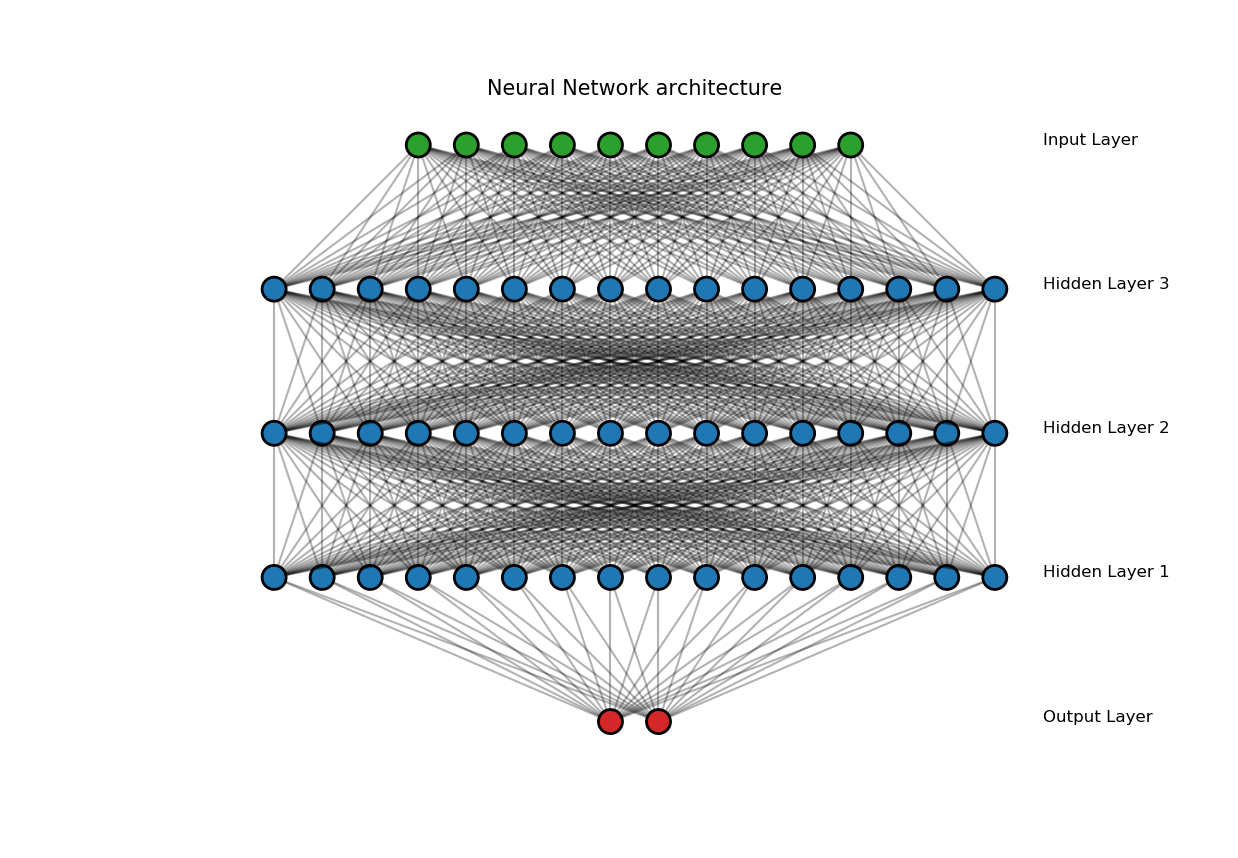
\includegraphics[width=\textwidth]{NN_NextStep_v2}
	\caption{Architektur Neuronales Netz für die NextStep Prädiktion}
	% \todo{Quelle Bild!}
	\label{fig:netArchitectureNextStep}
\end{figure}

\begin{figure}
    \centering
    \missingfigure{Grafik architektur Separator}
	% 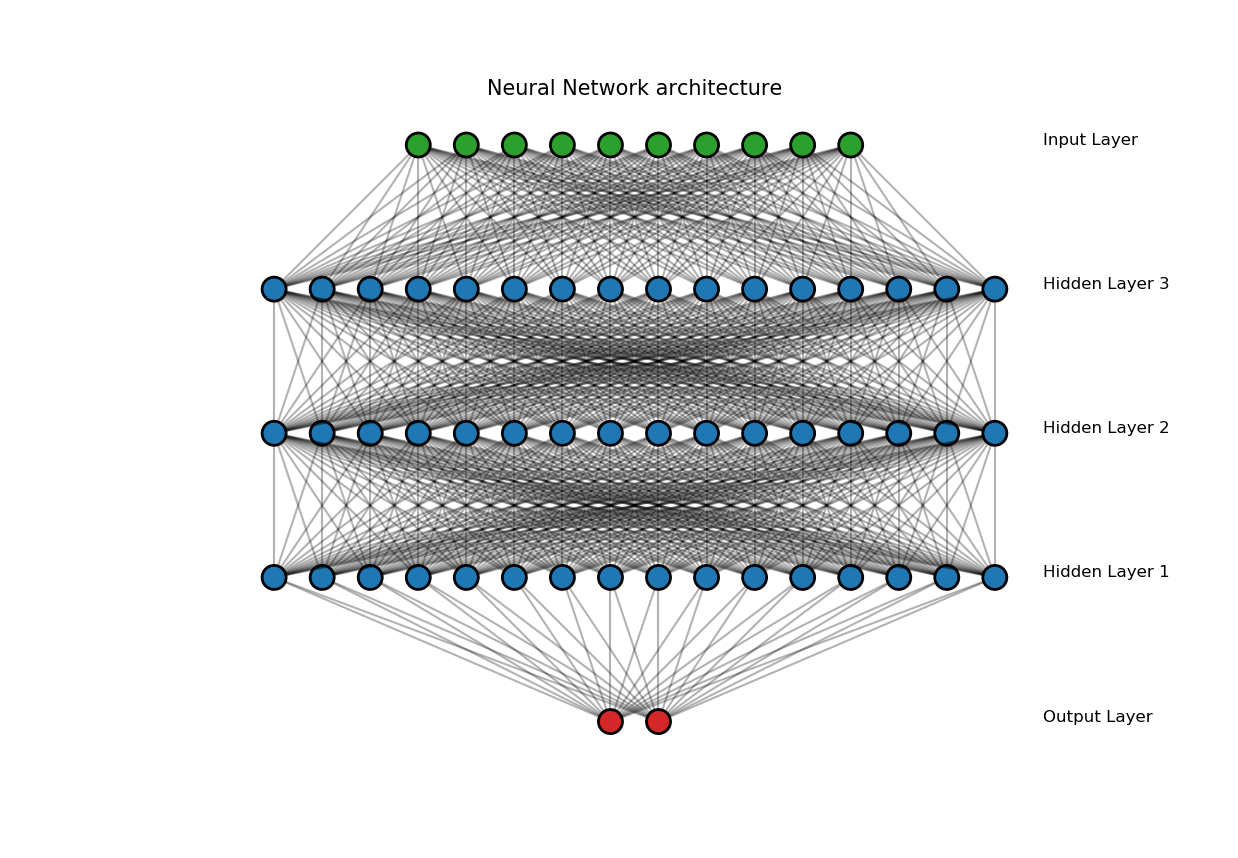
\includegraphics[width=\textwidth]{NN_NextStep_v2}
	\caption{Architektur Neuronales Netz für die Separator Prädiktion}
	% \todo{Quelle Bild!}
	\label{fig:netArchitectureSep}
\end{figure}
